\chapter{Introduzione}
\label{Introduzione}

L'introduzione deve presentare il lavoro in maniera chiara, deve contenere una breve descrizione del contesto, il lavoro che si andrà a svolgere e le ipotesi di partenza. 

\section{Inquadramento generale}
La prima parte contiene una frase che spiega l'area generale dove si svolge il lavoro; una che spiega la sottoarea più specifica dove si svolge il lavoro e la terza, che dovrebbe cominciare con le seguenti parole "lo scopo della tesi è ...", illustra l'obbiettivo del lavoro. Poi vi devono essere una o due frasi che contengano una breve spiegazione di cosa e come è stato fatto, delle attività sperimentali, dei risultati ottenuti con una valutazione e degli sviluppi futuri. La prima parte deve essere circa una facciata e mezza o due

\section{Breve descrizione del lavoro}
La seconda parte deve essere una esplosione della prima e deve quindi mostrare in maniera più esplicita l'area dove si svolge il lavoro, le fonti bibliografiche più importanti su cui si fonda il lavoro in maniera sintetica (una pagina) evidenziando i lavori in letteratura che presentano attinenza con il lavoro affrontato in modo da mostrare da dove e perché è sorta la tematica di studio. Poi si mostrano esplicitamente le realizzazioni, le direttive future di ricerca, quali sono i problemi aperti e quali quelli affrontati e si ripete lo scopo della tesi. Questa parte deve essere piena (ma non grondante come la sezione due) di citazioni bibliografiche e deve essere lunga circa 4 facciate.

\section{Struttura della tesi}
La terza parte contiene la descrizione della struttura della tesi.

\section{Come usare LaTeX}
Per creare i titoli delle sezioni presenti nell'introduzione va usato il comando "section", e per le successive sottosezioni "subsection". LaTeX adotta una logica ramificata, si possono quindi creare sottosezioni all'infinito aggiungendo il prefisso "sub".

Per separare due paragrafi basta lasciare un rigo vuoto come in questo caso. LaTeX, aggiungerà automaticamente un’indentazione.

A seguire sono presenti alcune sottosezioni contenenti informazioni su come usare le principali funzionalità di LaTeX.

\subsection{Sottosezione di esempio}
\subsubsection{Sotto-sottosezione di esempio}
\paragraph{Paragrafo}
\subparagraph{Sottoparagrafo}

\subsection{Riferimenti}

Una delle peculiarità di LaTeX è la gestione dei riferimenti, si basa sulla creazione di librerie contenenti le informazioni dei riferimenti. La libreria per la tesi si trova nel file "references.bib", al suo interno sono presenti ad ora solo tre riferimenti. Per aggiungere un testo alla libreria basta cercarlo su \url{www.bibtexsearch.com} oppure su \url{www.scholar.google.com}, copiare il suo identificativo BibTeX e incollarlo nella libreria. Se per un articolo non esiste l’identificativo BibTeX potete crearlo manualmente.

Ogni riferimento presente nella libreria presenta un “nome” con il quale va richiamato nel testo, questo è il codice presente sulla prima riga. Ad esempio, per citare \cite{greenwade93} basta richiamare con il comando "cite" il nome del riferimento, in questo caso “greenwade93”.

\subsection{Equazioni}
Le equazioni vanno scritte tra i comandi "begin equation" e "end equation", ad ogni equazione è bene assegnare un “nome” univoco con il comando "label" cosi da poterla richiamarla nel testo.

Per scrivere agevolmente le equazioni si può utilizzare il tool in bibliografia \cite{codecogs}, mentre per richiamarle nel testo basta utilizzare il loro nome e il comando “eqref”, come ad esempio con l'equazione \eqref{eq:equazioneEsempio}. 

\begin{equation} 
\label{eq:equazioneEsempio}
\int_{i=1}^{N}10x_{20}=\gamma \frac{10}{b_{10}^{4}}, \quad \forall i
\end{equation}
Equazioni troppo lunghe possono essere spezzate usando il comando multline:
\begin{multline}
J_i(x_{i},\boldsymbol {x}_{-i} ,\boldsymbol {\bar{\omega}})  =\sum_{h=1}^{H} K_{h} (\boldsymbol l_{-i}(h) + e_i(h) + \delta^{T} x_{i}(h)- \bar{\omega}(h)) \cdot 
\\
 \cdot (e_i(h) +\delta^{T} x_{i}(h))  + \sum_{h=1}^{H} W_{i} (\delta_{g}^{T} x_{i}(h))
\label{eq:equazioneEsempioLunga}
\end{multline}
Attenzione, le formule e le variabili possono anche essere inserite all'interno del testo utilizzando due simboli del dollaro come per esempio $f = \sum_d k$.

\subsection{Algoritmi}
Ecco un esempio di algoritmo:
\begin{algorithm}[H]
\caption{Nome dell'algoritmo}
\begin{algorithmic}
\STATE $\lambda^{+} = \mathrm{proj}_{\mathbb{R}^m_{\geq 0}}\left [ \lambda +\gamma \left (2A\boldsymbol{x}^{+}-A\boldsymbol{x}-b \right ) \right ]$
\FOR{$i = 1, ..., N$}
\IF {$i \in \mathcal{N_D}$}
\STATE Calculate $\boldsymbol{\bar{\omega}}$
\ELSIF {$i \in \mathcal{N_S}$}
\STATE Set $\hat{J}_i^M$ 
\ENDIF
\ENDFOR
\end{algorithmic}
\end{algorithm} 

\subsection{Elenchi }
Per inserire degli elenchi puntati va usato il comando "itemize", in questo modo:
\begin{itemize}
\item primo;
\item ultimo.
\end{itemize}
oppure per elechi numerati:
\begin{enumerate}
\item primo;
\item ultimo.
\end{enumerate}

\subsection{Tabelle}
Per presentare alcuni dati può essere utile inserire una tabella, darle un “nome” univoco e richiamarla nel testo in questo modo Tab. \ref{tab:tabellaEsempio}. Anche in questo caso vi è un ottimo tool per la creazione di tabelle \cite{CreateLaTexTable}.

\begin{table}[h]
\begin{center}
\caption{Titolo tabella}
\label{tab:tabellaEsempio}
\begin{tabular}{cccc}
        &  Top  & Bottom  &  Left/Right  \\
\hline
First   &  3.5  &  2.5    &     1.5      \\
Rest    &  2.5  &  2.5    &     1.5      \\ 
\hline
\end{tabular}
\end{center}
\end{table}


\subsection{Immagini}
Per aggiungere un’immagine basta caricarla nella cartella “02-figures” e caricarla nel testo come nell'esempio. LaTeX posizionerà automaticamente l'immagine nel testo, cercando la posizione ottimale. Anche per le immagini conviene usare un nome univoco come ad esempio in Fig.~\ref{fig:Prova1}. Può essere utile inserire una tilde ~ tra la parola Fig. e il riferimento, questo farà in modo di non spezzare il riferimento andando a capo. La stessa immagine può essere inserita a larghezza massima, come in Fig.~\ref{fig:Prova2}.
\begin{figure}[t!]
\centering
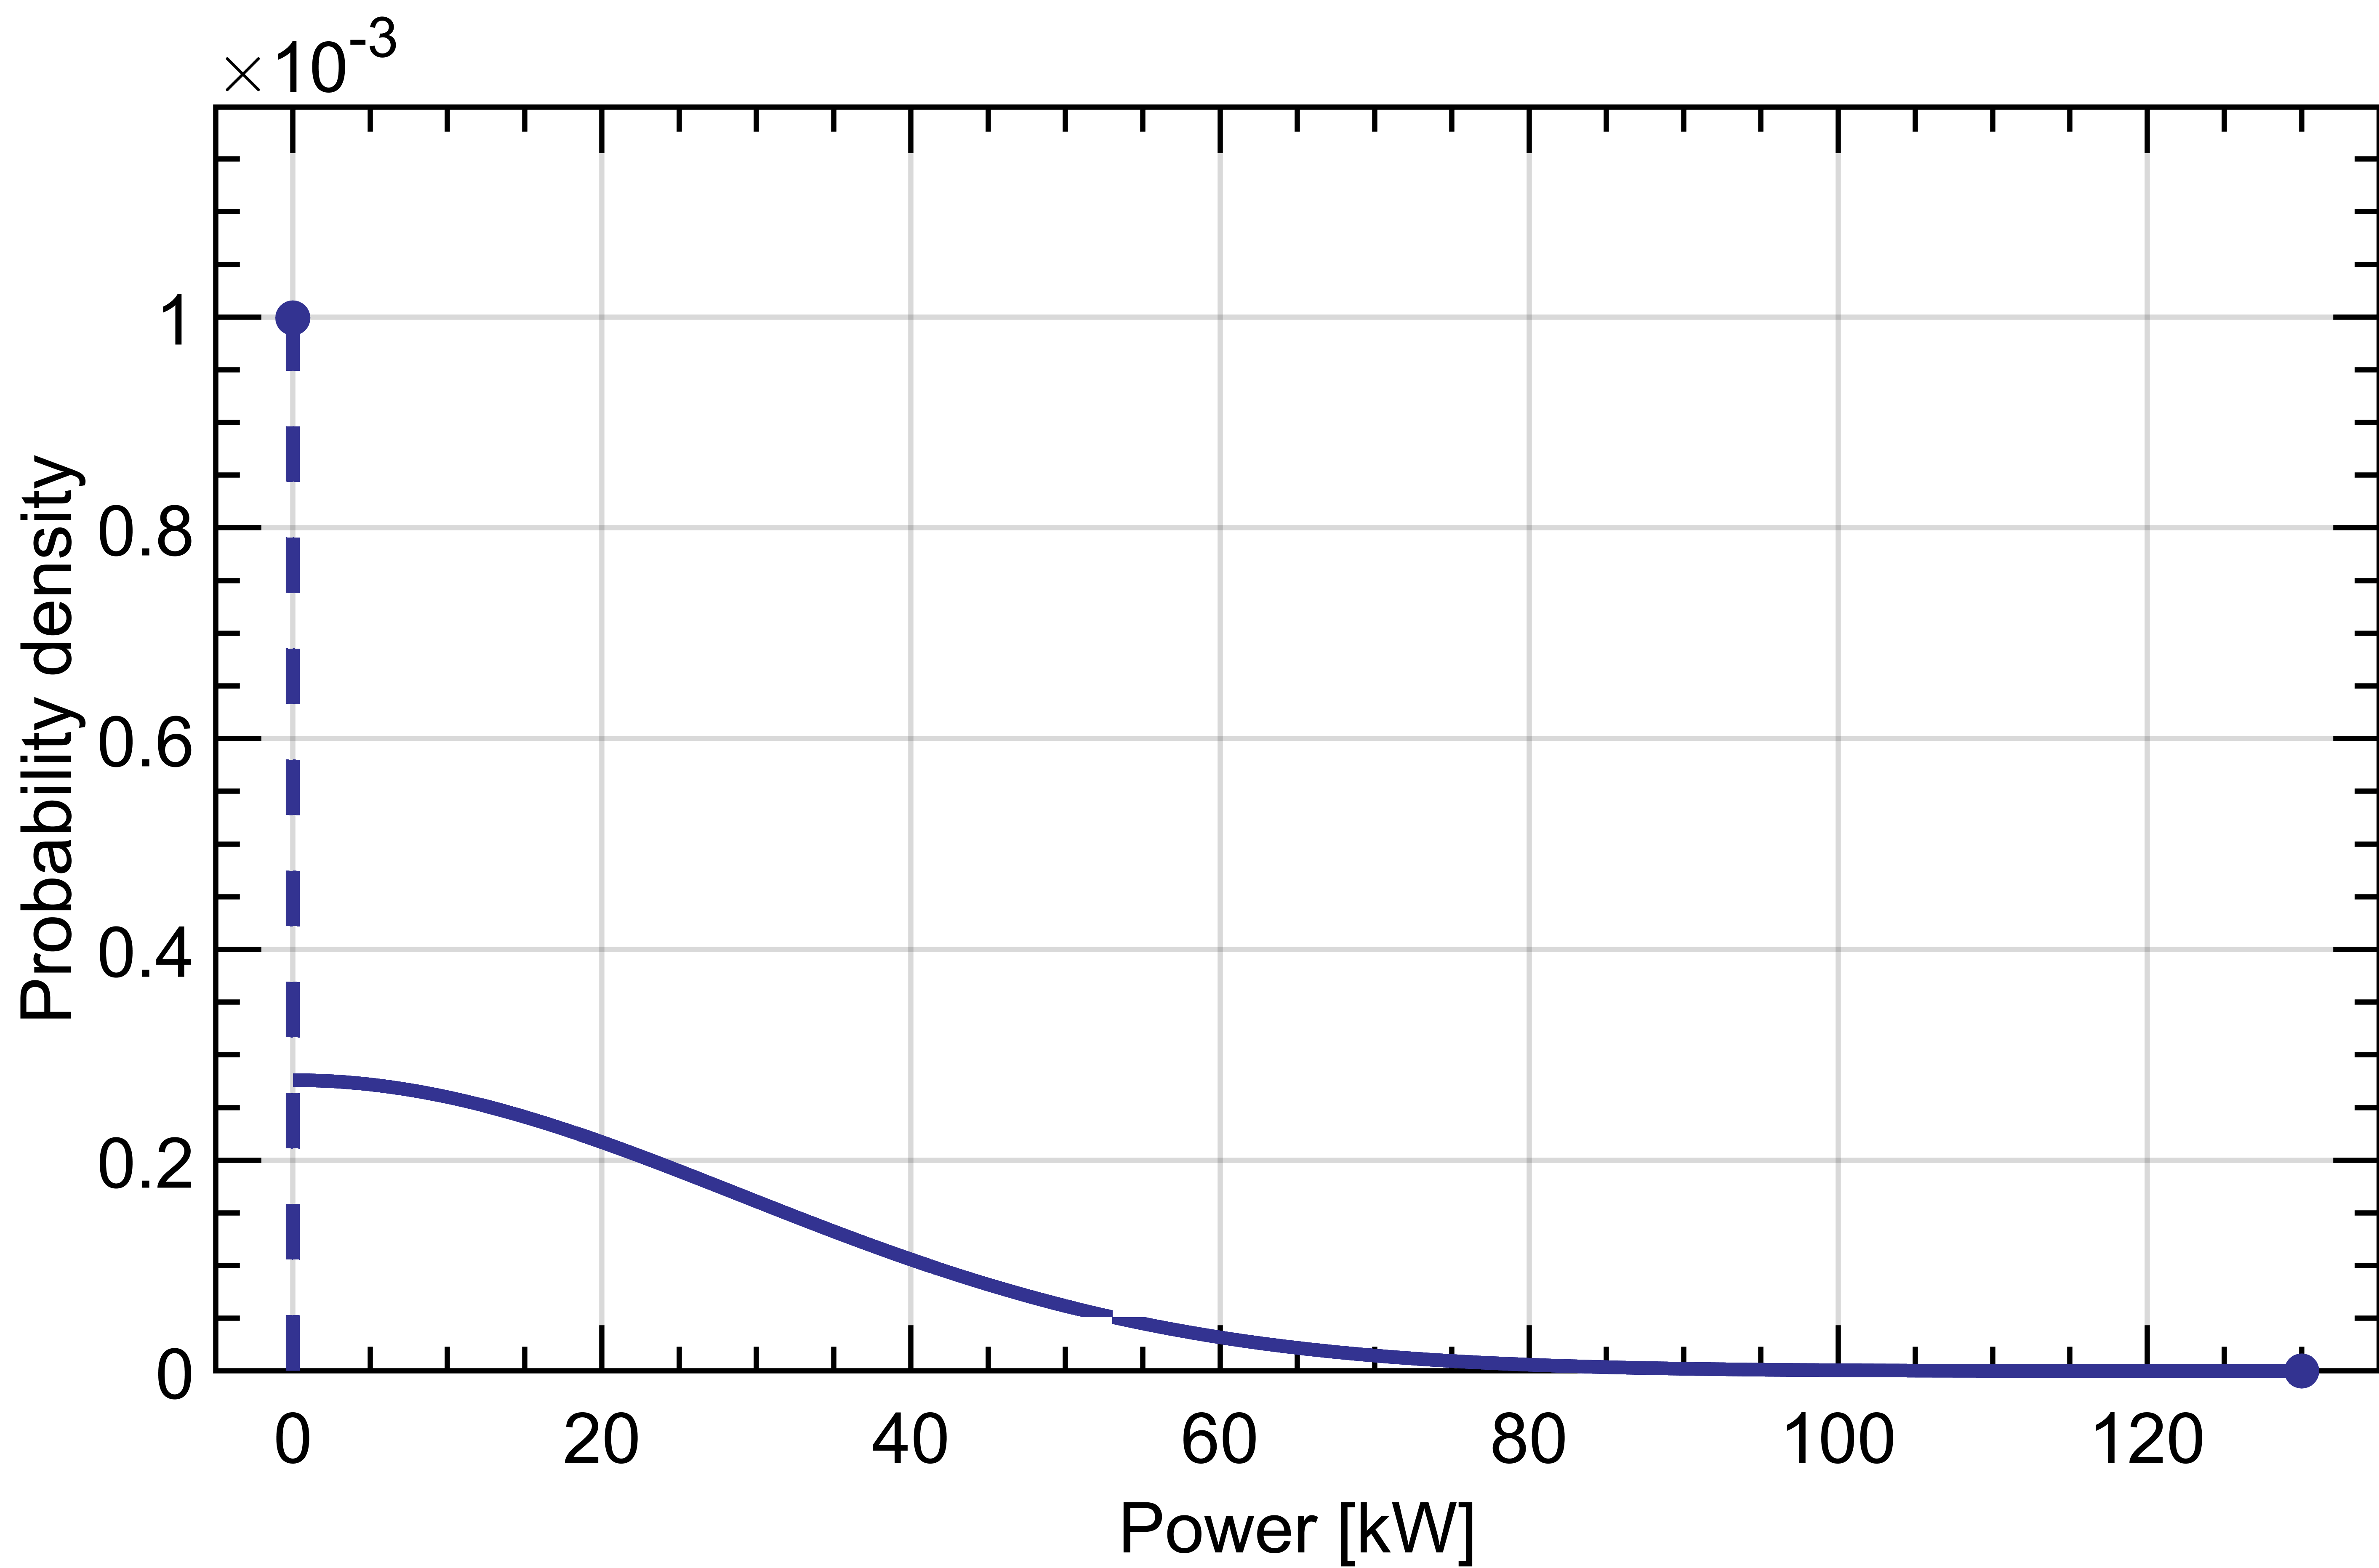
\includegraphics[width=0.4\textwidth]{02-figures/esempioFigura.png}
\caption{Esempio figura.}
\label{fig:Prova1}
\end{figure}

\begin{figure}[t!]
\centering
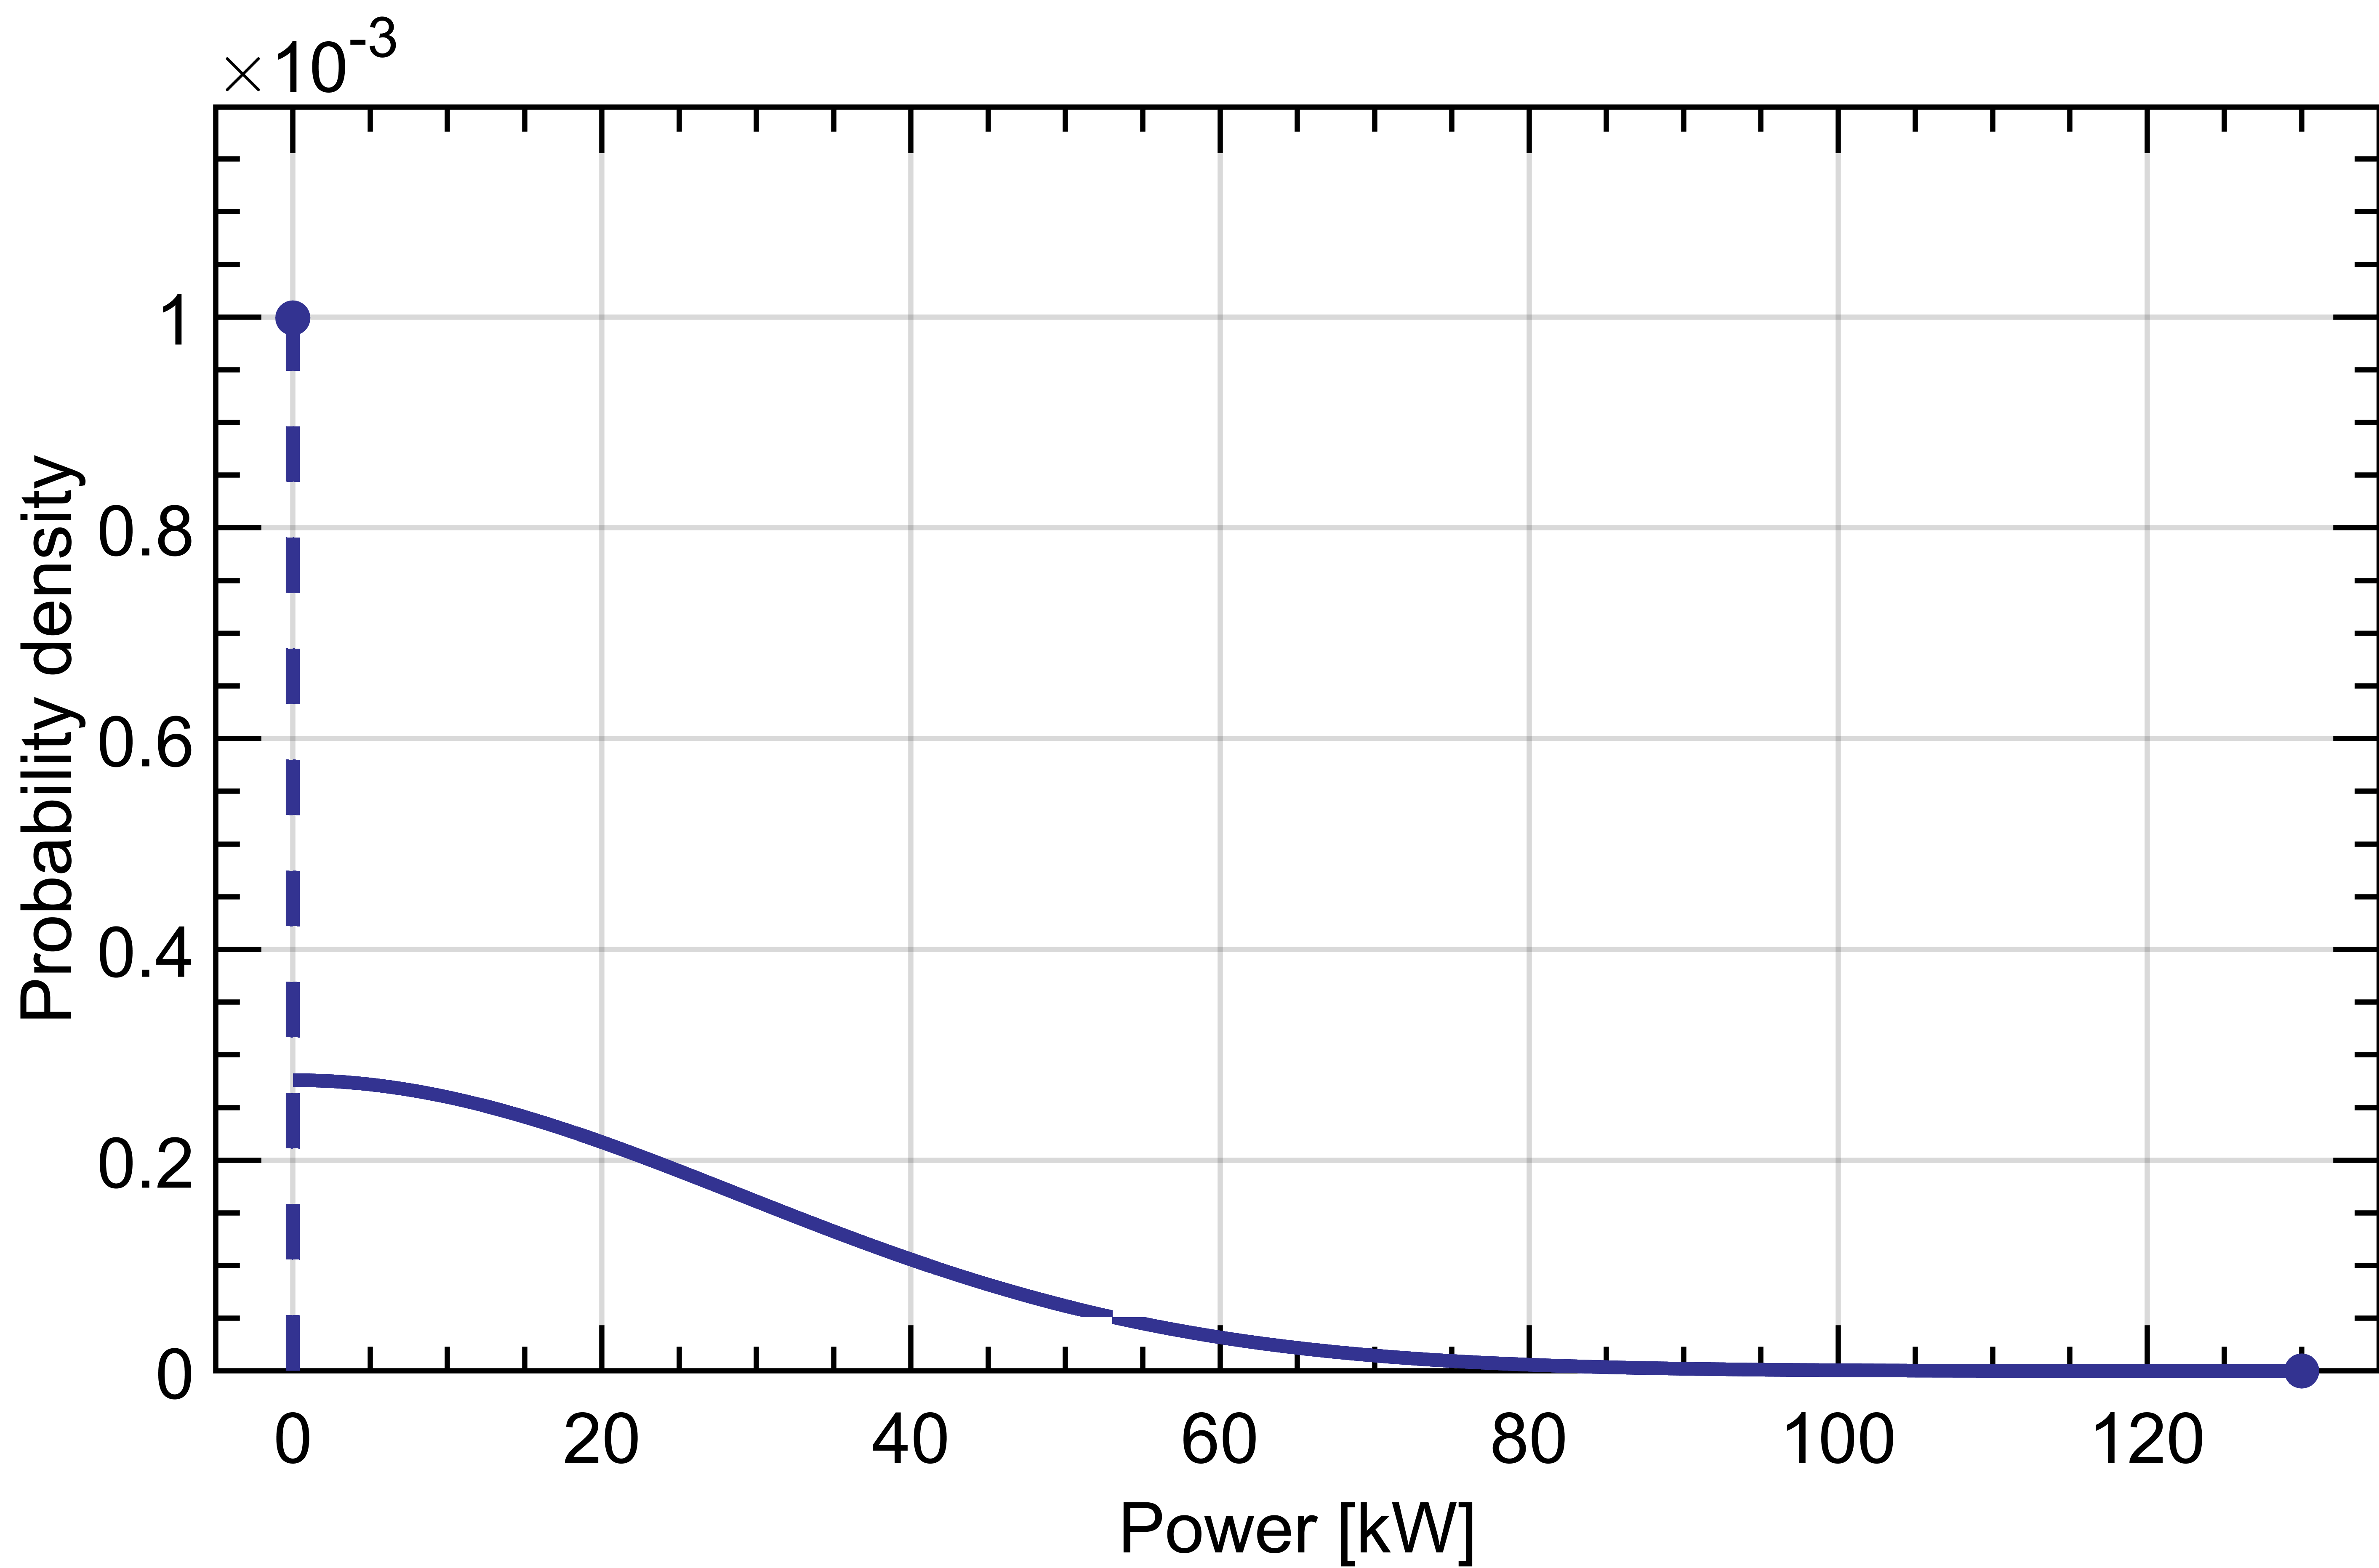
\includegraphics[width=1\textwidth]{02-figures/esempioFigura.png}
\caption{Esempio figura.}
\label{fig:Prova2}
\end{figure}

\newpage
\begin{figure}[H]
\centering
\subfloat[]{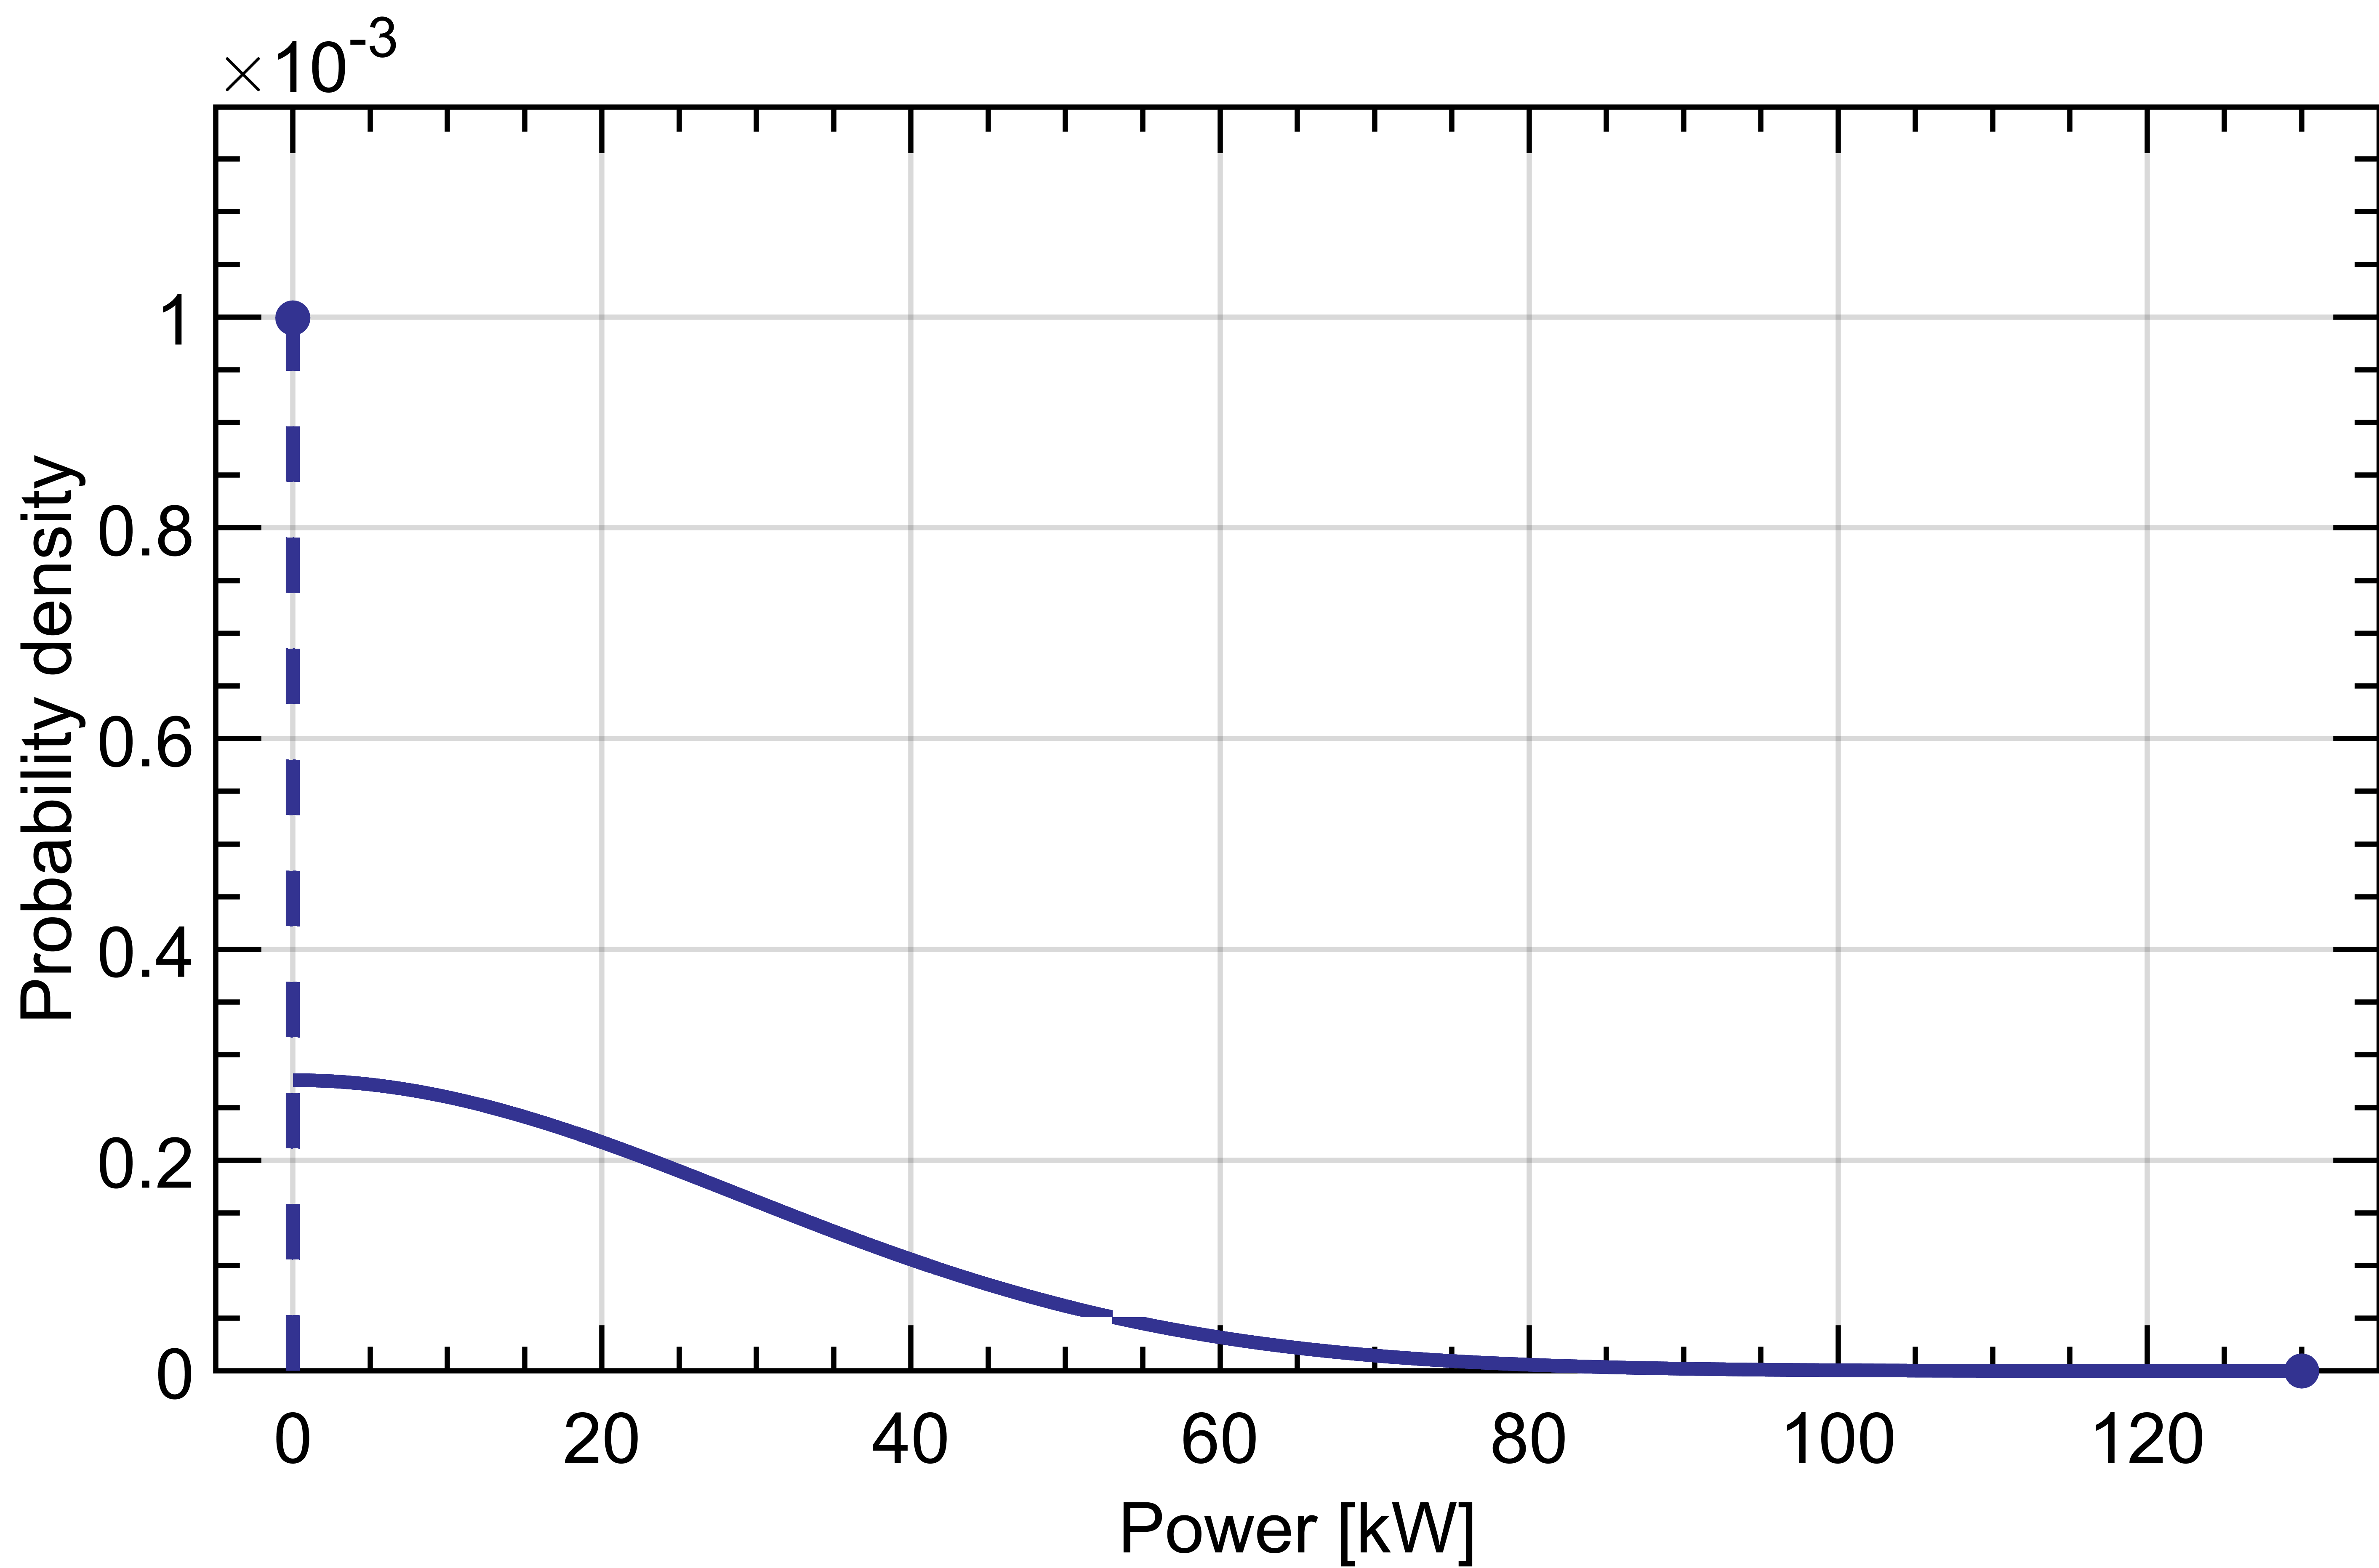
\includegraphics[width=0.45\textwidth]{02-figures/esempioFigura.png}}\hspace{0.1cm}
\subfloat[]{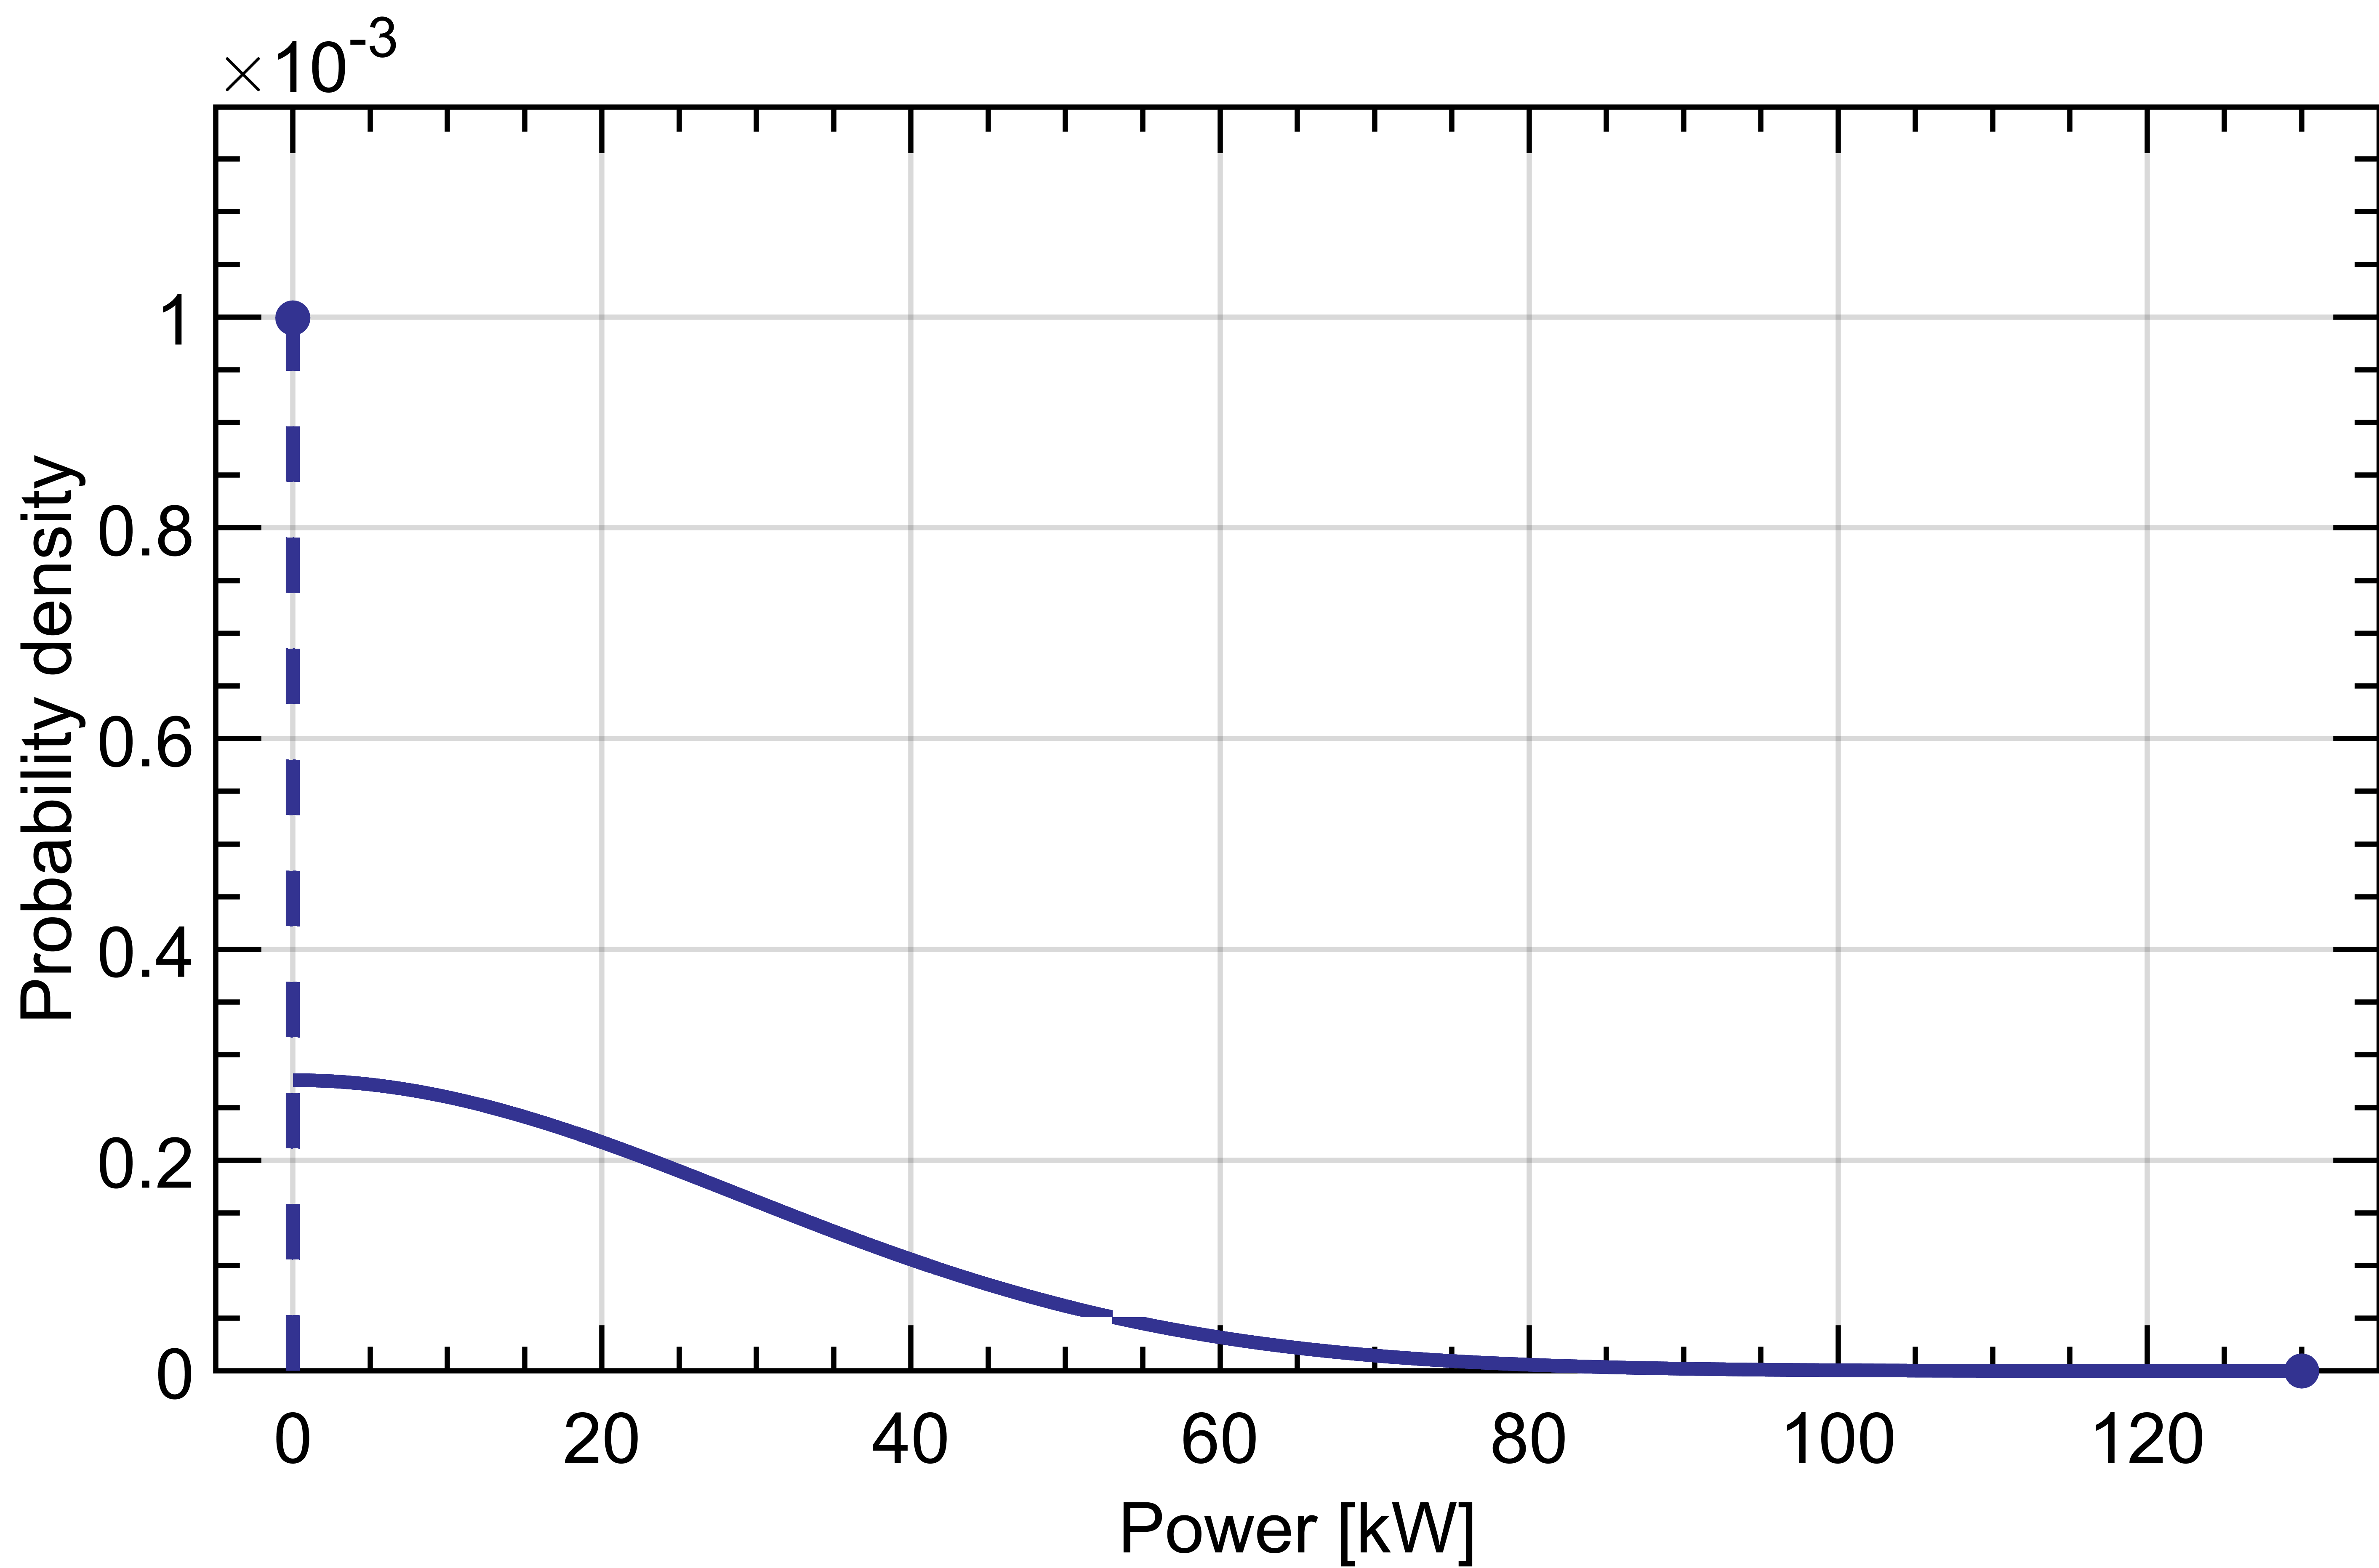
\includegraphics[width=0.45\textwidth]{02-figures/esempioFigura.png}}  \\
\caption{Esempio: (a) ..... e (b) .....}
\label{fig:5}
\end{figure}

Usare figure in .jpg o .png aumenta le dimensioni del file e ne riduce la qualità di stampa. Una soluzione può essere l'utilizzo di immagini in .pdf se sono schemi costruiti in Powerpoint oppure in .eps se figure generate in Matlab.
La figura \ref{fig:Prova1} è posizionata in alto, questo poiché è stato utilizzato il comando "t!". Per una panoramica sulle opzioni relative al posizionamento di figure, tabelle e algoritmi consultare \url{https://it.overleaf.com/learn/latex/Positioning_of_Figures}.

\begin{figure}[H]
\centering
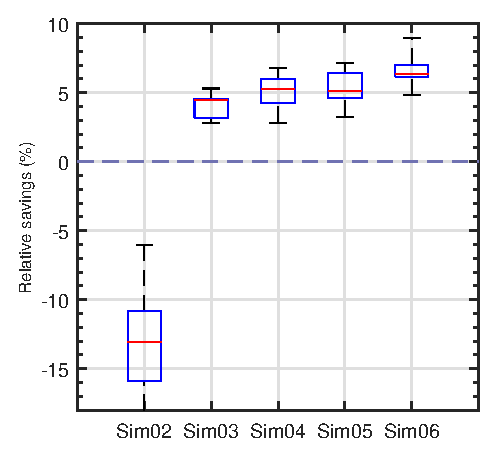
\includegraphics[width=0.6\textwidth]{02-figures/esempioFigura2.eps}
\caption{Esempio figura in formato eps.}
\label{fig:Prova3}
\end{figure}

\begin{figure}[H]
\centering
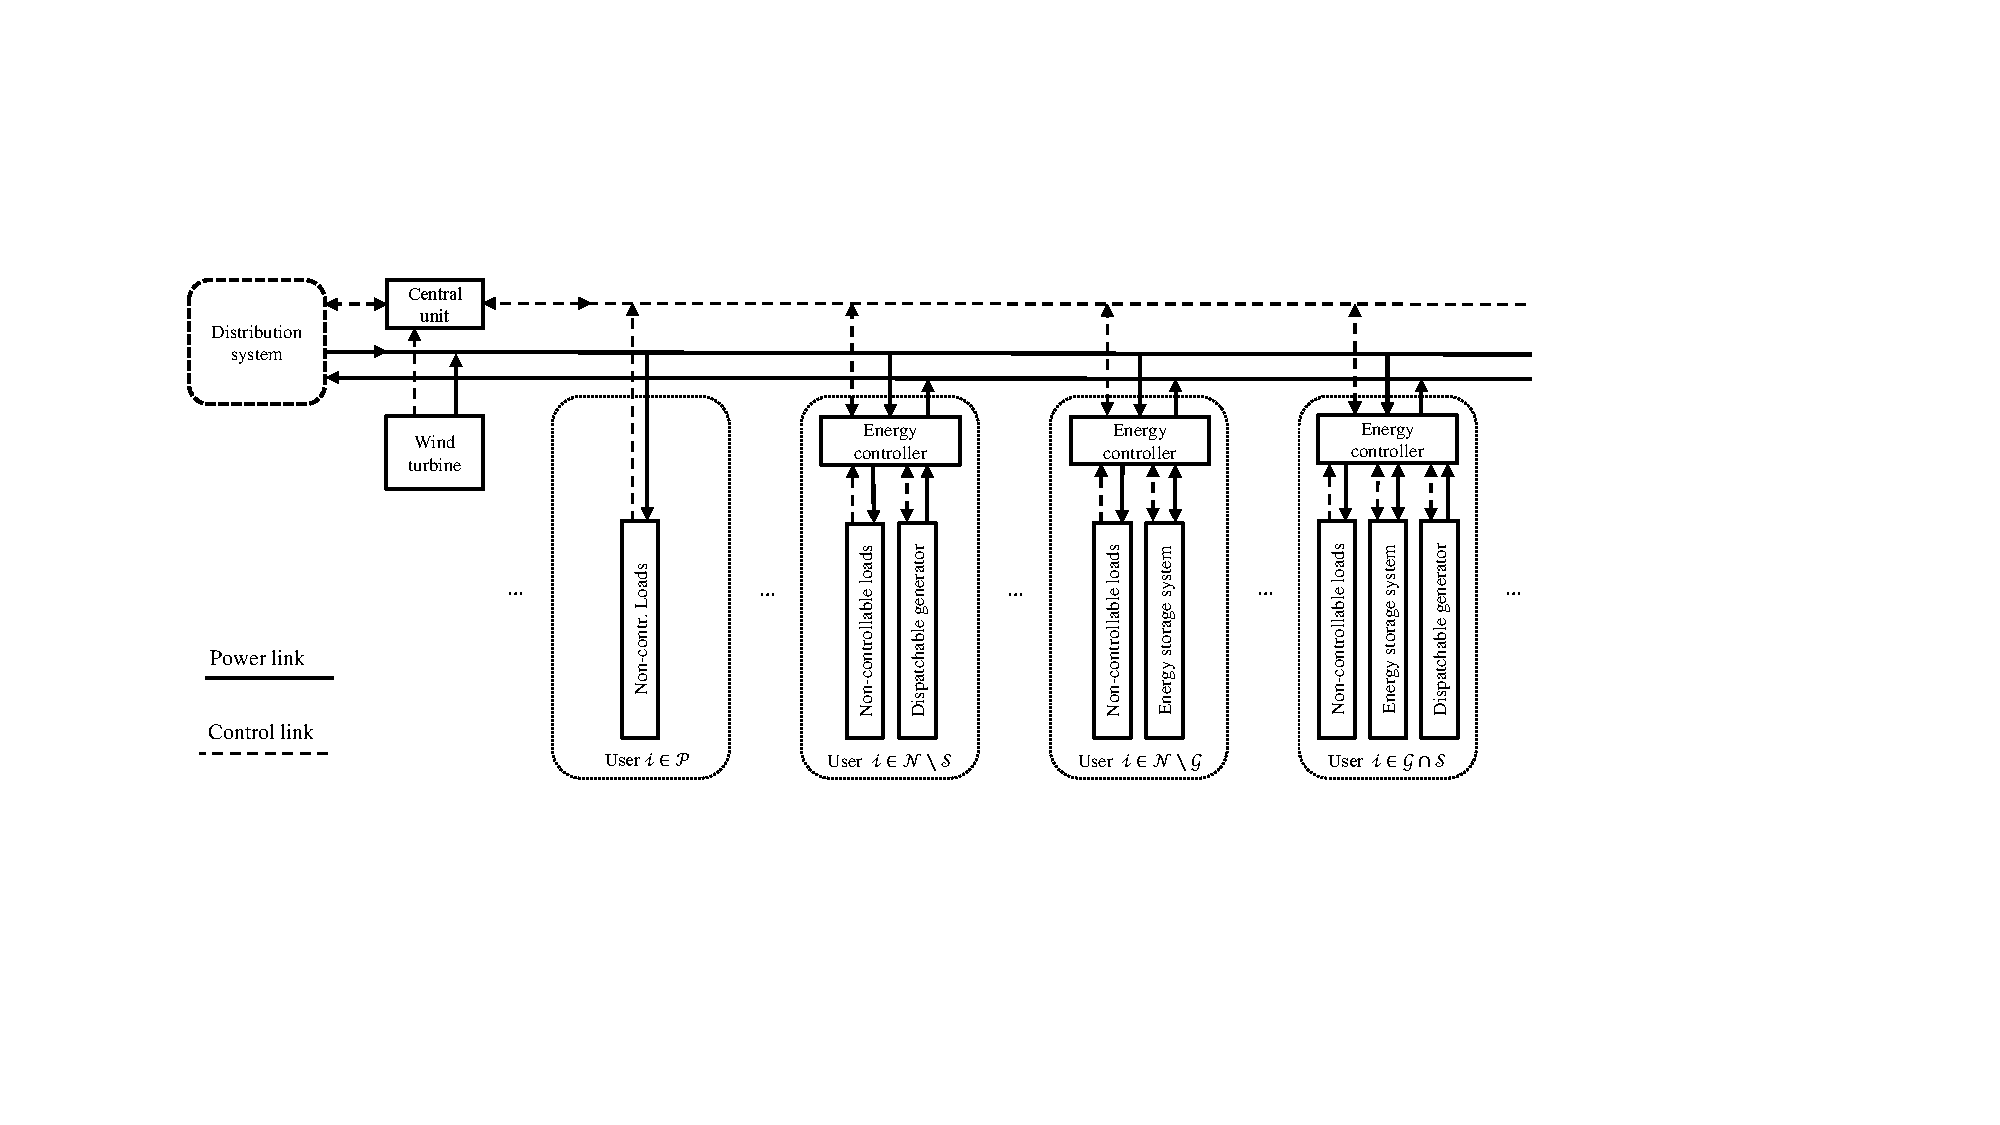
\includegraphics[width=\textwidth]{02-figures/esempioFigura3.pdf}
\caption{Esempio figura in pdf.}
\label{fig:Prova4}
\end{figure}

\subsection{Teoremi, definizioni, ecc.}
Il modello mette a disposizione gli ambienti "teorema", "definizione", "lemma" e "corollario", numerati automaticamente.
\begin{teorema}
Enunciato del teorema.
\end{teorema}

\begin{definizione}
Enunciato della definizione.
\end{definizione}

\begin{lemma}
Enunciato del lemma.
\end{lemma}

\begin{corollario}
Enunciato del corollario.
\end{corollario}


\begin{lstlisting}[language=Python]
    
\end{lstlisting}